\chapter[Идентификация нелинейных стохастических систем второго типа]{%
  Идентификация нелинейных стохастических систем второго типа
}

\section{Математическая модель идентифицируемой системы}

Для обеспечения наглядности сравнения рассматривался случай идентификации скалярной системы:
\begin{equation}
  \label{eq:nonlinear_model_scalar}
  \begin{aligned}
  h &= \psi(\overline{\theta}, \xi), \\
  x &= \xi + \varepsilon_x, \\
  y &= h + \varepsilon_y,
  \end{aligned}
\end{equation}
где \( \xi, h \) "--- фактические значения входной и выходной переменной, \par
\( \psi \) "--- скалярно-векторная функция регрессии, \par
\(
\overline{\theta} = (\theta_1, \theta_2, \dotsc, \theta_m)
\) "--- вектор фактических значений параметров объекта, \par
\( x, y \) "--- измеренные значения входной и выходной переменной, \par
\( \varepsilon_x, \varepsilon_y \) "--- независимые ошибки измерений значений входной и
выходной переменной, распределенные по нормальному закону:
\(
\varepsilon_x = N(0, \sigma_{\varepsilon_x}),
\varepsilon_y = N(0, \sigma_{\varepsilon_y})
\).

\section{Алгоритмы методов идентификации}

\subsection{Нелинейный метод наименьших квадратов}

Один из подходов к оценке параметров системы~\eqref{eq:nonlinear_model_scalar} состоит в следующем.
Можно <<закрыть глаза>> на существование ошибок измерений
входной переменной, то есть считать, что \( \varepsilon_x = 0 \),
и вместо данной модели рассматривать модель
\begin{equation}
  \label{eq:nonlinear_model_lse}
  \begin{aligned}
  x &= \psi(\overline{\theta}, \xi), \\
  y &= x + \varepsilon_y.
  \end{aligned}
\end{equation}

Тогда оценка вектора параметров объекта определяется выражением~\cite{mukha_2009}
\begin{equation}
  \label{eq:nonlinear_lse}
  \hat{\overline{\theta}}_{\text{НМНК}} =
  \overline{\theta}_0 + (Q^T R^{-1}_{\Xi} Q)^{-1} Q^T R^{-1}_{\Xi} (y - \psi(\overline{\theta}_0, x)),
\end{equation}
где \( \overline{\theta}_0 \) --- опорная точка,
\( Q = \dfrac{\partial \psi(\overline{\theta}_0, x) }{ \partial \overline{\theta}_0 } \).

Эту оценку будем называть оценкой, полученной нелинейным
методом наименьших квадратов (НМНК-оценкой).
В качестве опорной точки \( \overline{\theta}_0 \) можно использовать значения
\( \theta_1, \dotsc, \theta_m \),
полученные в результате численного решения системы уравнений
\begin{equation}
  \label{eq:nonlinear_basic}
  (y_j - \psi( \overline{\theta}, x_j )) = 0, \: j = \overline{1,m},
\end{equation}
где \( x_j, y_j \) --- опорные наблюдения входа и выхода системы соответственно.

В качестве опорных значений могут выступать, например:
\begin{itemize}
\item первые наблюдения:
  \[ (x_1, y_1), (x_2, y_2), \dotsc , (x_m, y_m); \]
\item равноотстоящие наблюдения:
  \[
    (x_{k}, y_{k}), (x_{2k}, y_{2k}) , \dotsc , (x_{mk}, y_{mk}), \:
    k = \lfloor \dfrac{n}{m} \rfloor;
  \]
\item усредненные наблюдения:
  \begin{gather*}
    ( \overline{x}_{k}, \overline{y}_{k} ),
    ( \overline{x}_{2k}, \overline{y}_{2k} ),
    \dotsc ,
    ( \overline{x}_{mk}, \overline{y}_{mk}), \\
    \overline{x}_{ik} = \dfrac{1}{m} \sum_{j = 1+(i-1)k}^{ik} x_j, \quad
    \overline{y}_{ik} = \dfrac{1}{m} \sum_{j = 1+(i-1)k}^{ik} y_j, \quad
    k = \lfloor \dfrac{n}{m} \rfloor.
  \end{gather*}
\end{itemize}

Для уточнения оценки, полученной по формуле~\eqref{eq:nonlinear_lse}, можно
организовать итерационную процедуру, заменяя опорную точку полученной оценкой.

\vspace{2\baselineskip}
\subsection{Метод рядов Тейлора}

Применение метода рядов Тейлора (МРТ)~\cite{mukha_2000}
требует иной формулировки задачи, допускаемой формулировкой \eqref{eq:nonlinear_model_scalar}.
Следует предположить, что \( j \)-е наблюдение вектора параметров \( \overline{theta}_j \)
определяется как векторная функция показаний приборов:
\begin{equation}
  \label{eq:nonlinear_mrt_phi}
  \overline{\theta}_j = \phi( \overline{z}_{j} ), \: j = \overline{1, n},
\end{equation}
где вектор
\( \overline{z}^{\text{T}}_{j} =
( \overline{x}^{\text{T}}_{j}, \overline{y}^{\text{T}}_{j}) \)
имеет нормальное распределение \( N(A_{z,j}, R_{z,j}) \)
и оцениваемый векторный параметр \( \overline{\theta} \) определяется как
\( \overline{\theta} = \phi(A_{z,j}), \forall i = \overline{1, n} \).
В этом случае МРТ-оценка \( \hat{\overline{\theta}}_{\text{МРТ}} \) векторного параметра \( \overline{\theta} \)
определяется выражением
\begin{equation}
  \label{eq:nonlinear_mrt}
  \hat{\overline{\theta}}_{\text{МРТ}} =
  \Bigg( \sum^{n}_{i=1} R^{-1}_{\theta,i} \Bigg)^{-1}
  \sum^{n}_{j=1} R^{-1}_{\theta,j} \overline{\theta}_j,
\end{equation}
где
\( R_{\theta,i} = G_i R_{z,i} G^T_i \),
\( G_i =
\dfrac{\partial \phi( \overline{z}_{i} ) }{ \partial \overline{z}_{i} } \).

Численное значение наблюдения \( \theta_j \)~\eqref{eq:nonlinear_mrt_phi} может определяться как
решение системы уравнений~\eqref{eq:nonlinear_basic}.


\section{Численный анализ точности оценивания параметров}

\subsection{Методика сравнения}

Было выполнено сравнение точности оценок,
полученных нелинейным методом наименьших квадратов и методом рядов Тейлора,
для функций регрессии различного вида,
в зависимости от с.~к.~о ошибок измеряемых значений
\( \sigma_{\varepsilon_x}, \sigma_{\varepsilon_y} \).

В качестве величины, характеризующей сравнительную точность оценивания параметров,
использовалась разность средних Евклидовых расстояний
между точными значениями параметров модели и их оценками, полученными
с помощью НМНК и МРТ:
\begin{equation}
  \begin{aligned}
    d &= d_{\text{НМНК}} - d_{\text{МРТ}}, \\
    d_{\text{НМНК}} &=
    \frac{1}{k} \sum_{j=1}^k
    \sqrt{\sum_{\text{i=1}}^m (\hat{\theta}_{\text{НМНК}_{ij}} - \theta_{ij})^2}, \\
    d_{\text{МРТ}} &=
    \frac{1}{k} \sum_{j=1}^k
    \sqrt{\sum_{\text{i=1}}^m (\hat{\theta}_{\text{МРТ}_{ij}} - \theta_{ij})^2}.
  \end{aligned}
  \label{eq:dst_nonlinear_param}
\end{equation}
Таким образом, при \( d > 0 \) точность оценивания параметров модели с помощью МРТ
превосходит точность НМНК, а при \( d < 0 \) НМНК-оценки являются более точными.
При \( d = 0 \) оба метода дают оценки одинаковой точности.

Значения \( \xi_i \) выбирались из равномерного в \( [0, 10] \) распределения.
Для получения каждой оценки \( \hat{\overline{\theta}} \) использовались результаты
ста наблюдений \( ( x_i, y_i ), i = \overline{1, n}, n = 100 \).

Расчеты величины \( d \) производились в узлах сетки значений
\( \sigma_{\varepsilon_x}, \sigma_{\varepsilon_y} \) в прямоугольнике
\( [0, 2] \times [0, 2] \) с шагом 0{,}1.
В каждом узле сетки вычислялось \( k = 100 \) оценок.
Для расчета оценок использовались средние опорные наблюдения.
В качестве значений НМНК-оценки \( \theta_{\text{НМНК}} \)
использованы значения, полученные на первой итерации метода.

% \vspace{2\baselineskip}
% \subsection{Линейная функция регрессии}

% Частным случаем нелинейной модели~\eqref{eq:nonlinear_model_scalar} является линейная,
% то есть такая, функция регрессии которой имеет вид \( \psi = \theta_0 + \theta_1 \xi \).

% На рисунке~\ref{fig:comparison_nonlinear_linear}
% представлены графики функции \( d(\sigma_{\varepsilon_x}, \sigma_{\varepsilon_y}) \)
% при различных значениях параметра \( \theta_1 \).
% По результатам сравнения можно заключить, что точность оценивания параметров линейных моделей
% не зависят от постоянной составляющей \( \theta_0 \), и что оценки, полученные с помощью НМНК,
% являются более точными во всем диапазоне величин \( \theta_1 \).

% \begin{figure}[p]
%   \begin{subfigure}[b]{\linewidth}
%     \centering
%     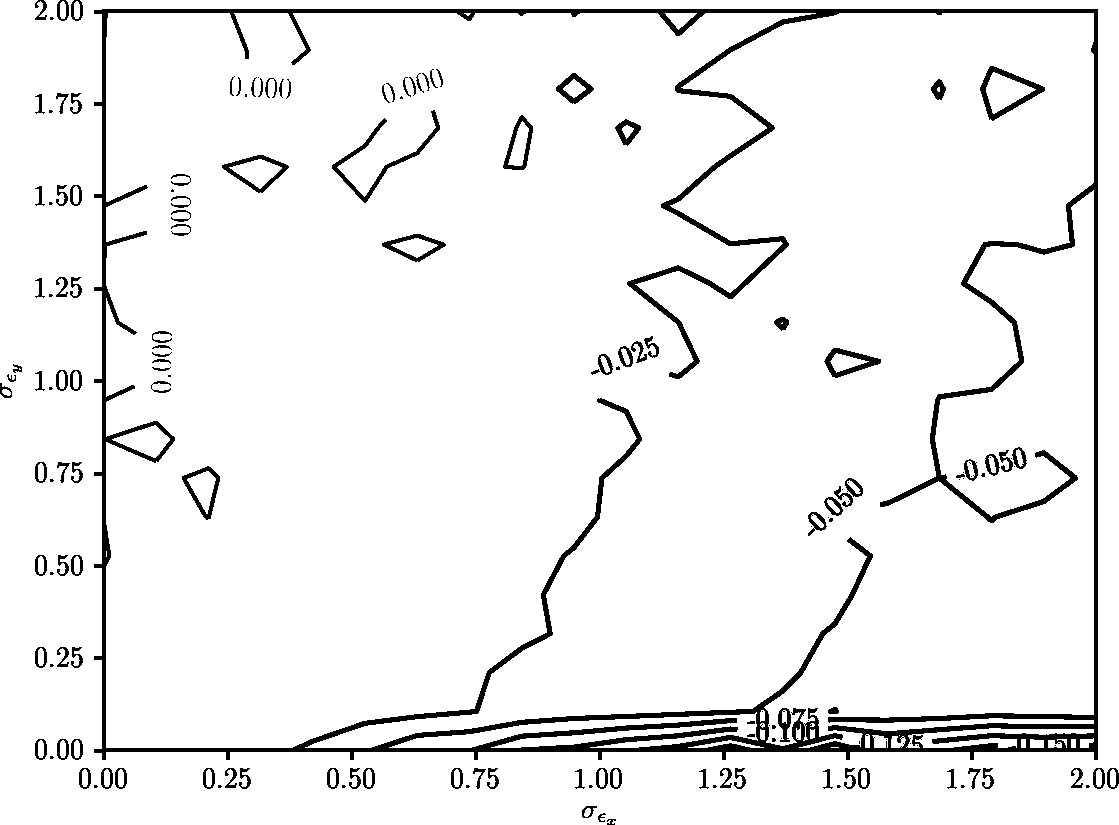
\includegraphics[width=135mm]{fig/nonlinear/linear/a-0_b-0,2.png}
%     \caption{\( \theta_1 = 0{,}2 \)}
%   \end{subfigure}

%   \vspace{2\baselineskip}
%   \begin{subfigure}[b]{\linewidth}
%     \centering
%     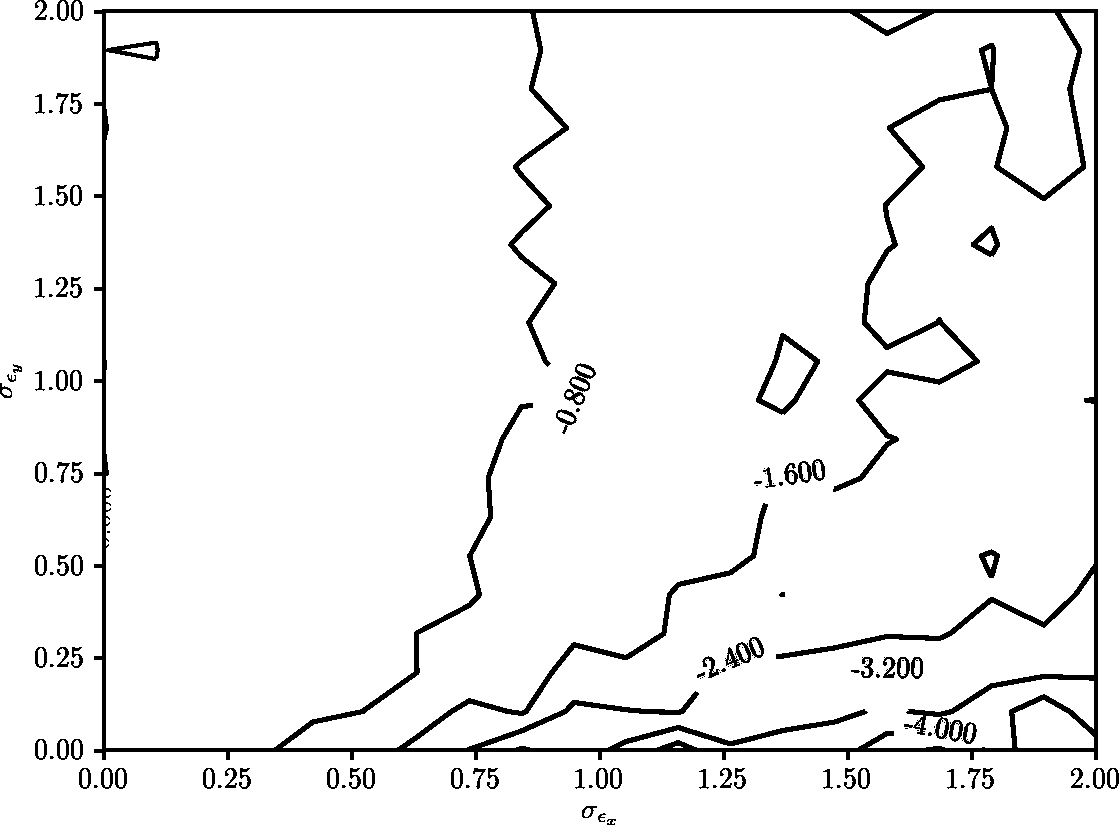
\includegraphics[width=135mm]{fig/nonlinear/linear/a-0_b-5.png}
%     \caption{\( \theta_1 = 5 \)}
%   \end{subfigure}

%   \vspace{\baselineskip}
%   \caption{%
%     Точность оценивания \\
%     параметров линейной модели
%   }\label{fig:comparison_nonlinear_linear}
% \end{figure}

\pagebreak
\subsection{Параболическая функция регрессии}

Параболическая функция регрессии вида
\( \psi = \theta_0 + \theta_1 \xi + \theta_2 \xi^2 \)
является, пожалуй, наиболее <<популярной>> из нелинейных.

На рисунках~\ref{fig:comparison_nonlinear_quadratic_a-0_b-0_c-1}--\ref{fig:comparison_nonlinear_quadratic_a-0_c-1} представлен ряд графиков зависимости \( d(\sigma_{\varepsilon_x}, \sigma_{\varepsilon_y}) \)
для параболической функции регрессии при различных значениях её параметров.
По результатам анализа данных графиков можно сделать следующие выводы:
\begin{enumerate}
\item Точность оценивания не зависит от фактического значения постоянной составляющей \( \theta_0 \).
\item Если функция регрессии на промежутке аппроксимации является монотонной,
  точность оценивания зависит главным образом от абсолютного значения параметра \( \theta_2 \)
  (рисунки~\ref{fig:comparison_nonlinear_quadratic_a-0_b-0_c-1},~\ref{fig:comparison_nonlinear_quadratic_a-0_b-0},~\ref{fig:comparison_nonlinear_quadratic_a-0_b-5_c-1}).
  При больших значениях данного параметра оценки, полученные НМНК,
  являются более точными, чем МРТ-оценки.
\item В случае, когда функция регрессии на промежутке аппроксимации является немонотонной,
  метод рядов Тейлора оценивает параметры модели более точно, чем НМНК
  (рисунок~\ref{fig:comparison_nonlinear_quadratic_a-0_b--5_c-1}).
\end{enumerate}

\begin{figure}[b]
  \centering
  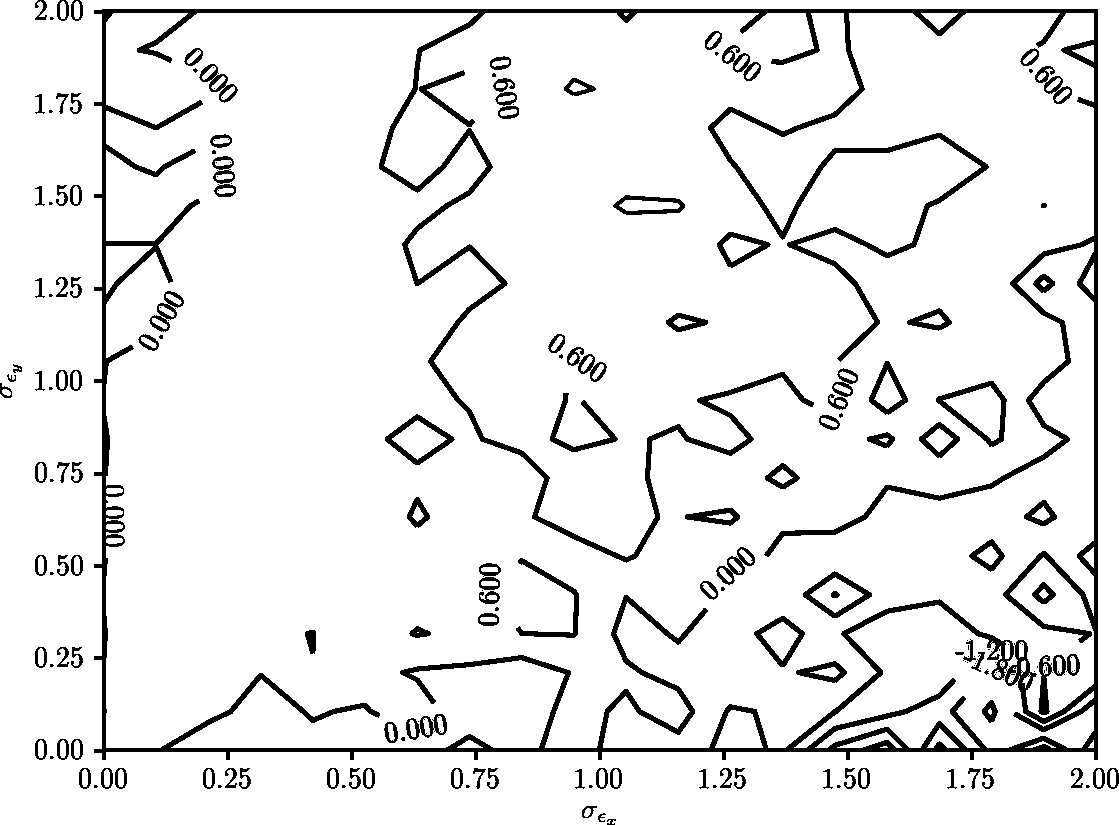
\includegraphics[width=135mm]{fig/nonlinear/quadratic/a-0_b-0_c-1.png}
  \caption{
    Точность оценивания параметров \\
    параболической модели при \( \theta_0 = 0, \theta_1 = 0, \theta_2 = 1 \)
  }\label{fig:comparison_nonlinear_quadratic_a-0_b-0_c-1}
\end{figure}

\begin{figure}[p]
  \begin{subfigure}[b]{\linewidth}
    \centering
    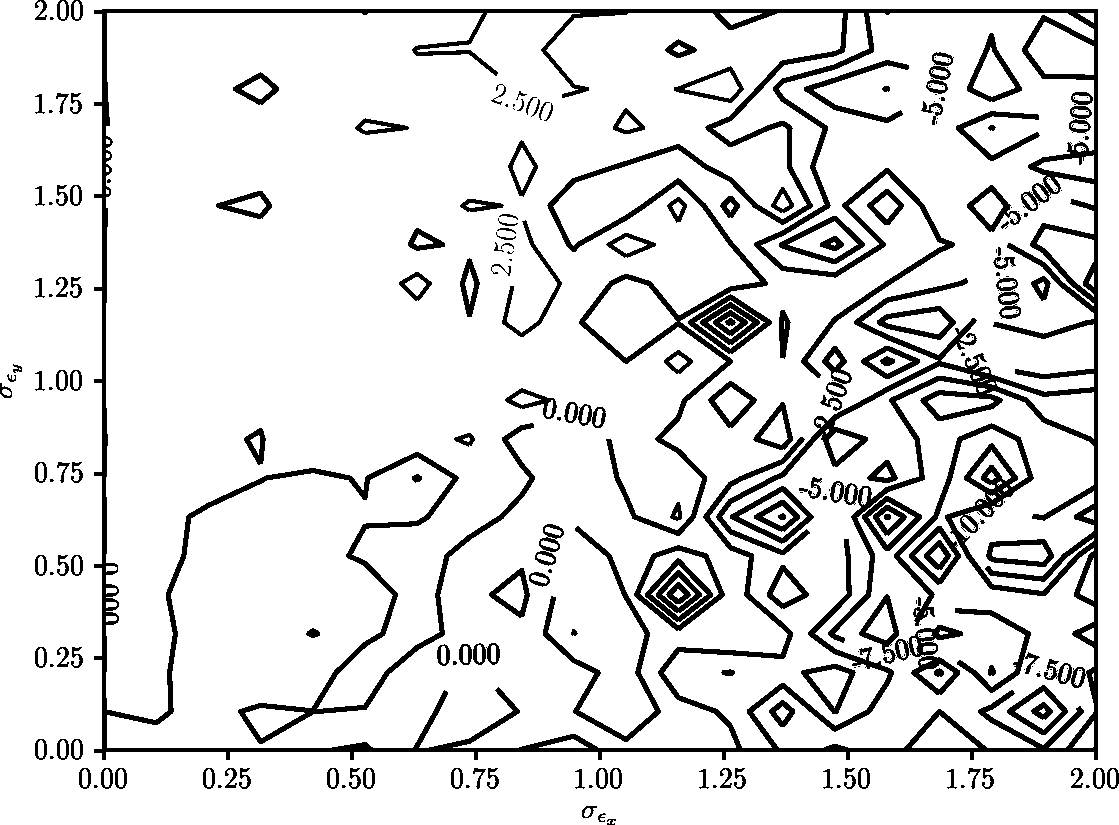
\includegraphics[width=135mm]{fig/nonlinear/quadratic/a-0_b-0_c--5.png}
    \caption{\( \theta_2 = -5 \)}
  \end{subfigure}

  \vspace{2\baselineskip}
  \begin{subfigure}[b]{\linewidth}
    \centering
    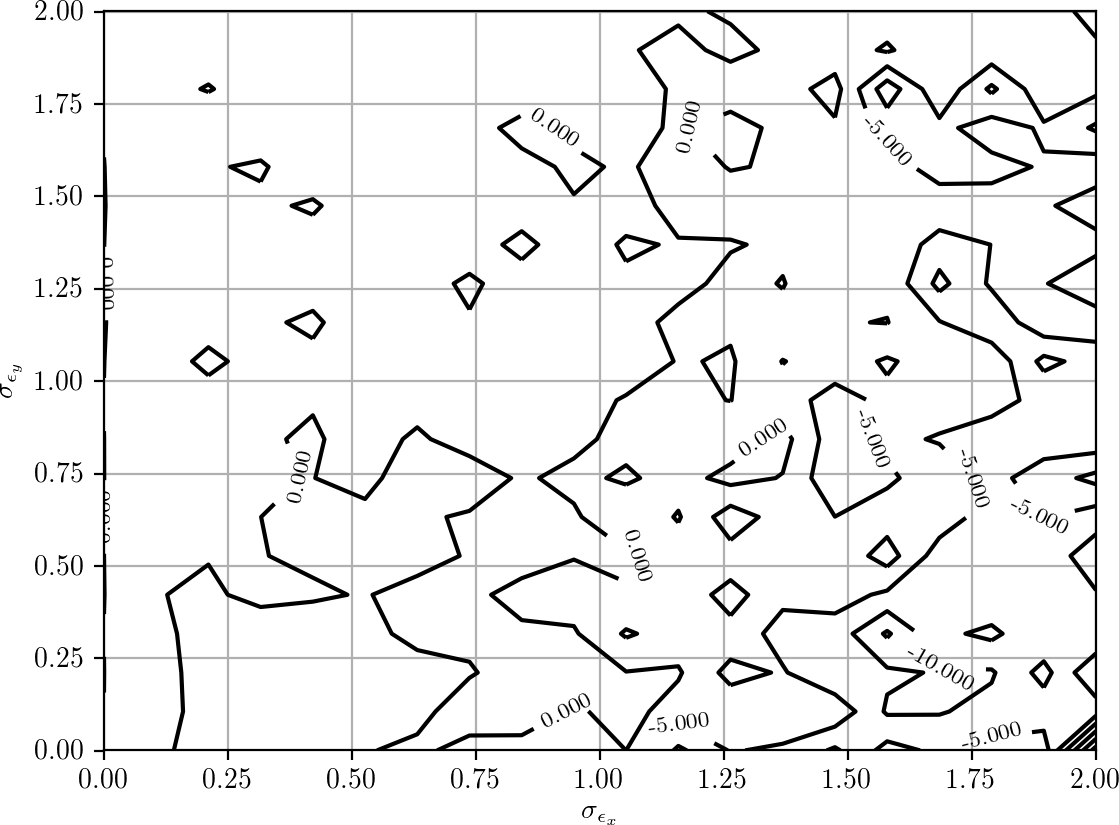
\includegraphics[width=135mm]{fig/nonlinear/quadratic/a-0_b-0_c-5.png}
    \caption{\( \theta_2 = 5 \)}
  \end{subfigure}

  \vspace{\baselineskip}
    \caption{
      Точность оценивания параметров \\
      параболической модели при \( \theta_0 = 0, \theta_1 = 0 \)
    }\label{fig:comparison_nonlinear_quadratic_a-0_b-0}
\end{figure}

\begin{figure}[p]
  \begin{subfigure}[b]{\linewidth}
    \centering
    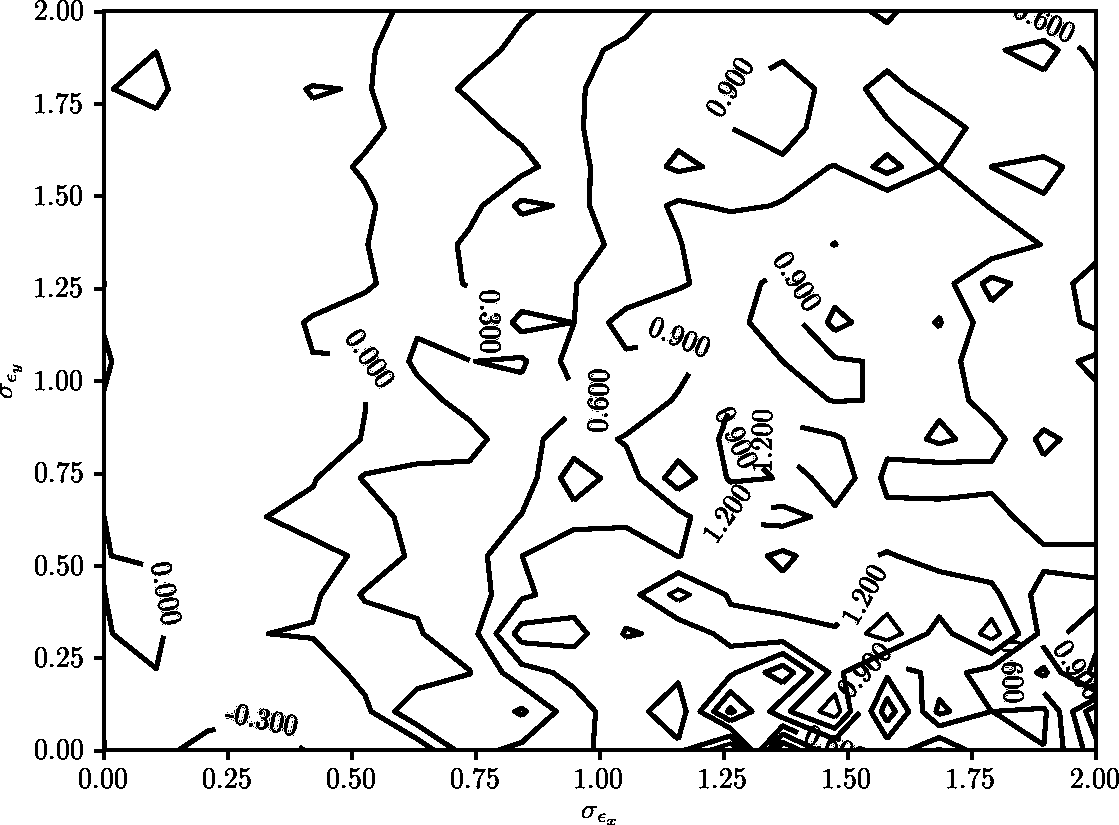
\includegraphics[width=135mm]{fig/nonlinear/quadratic/a-0_b--5_c-1.png}
    \caption{\( \theta_1 = -5 \)}\label{fig:comparison_nonlinear_quadratic_a-0_b--5_c-1}
  \end{subfigure}

  \vspace{2\baselineskip}
  \begin{subfigure}[b]{\linewidth}
    \centering
    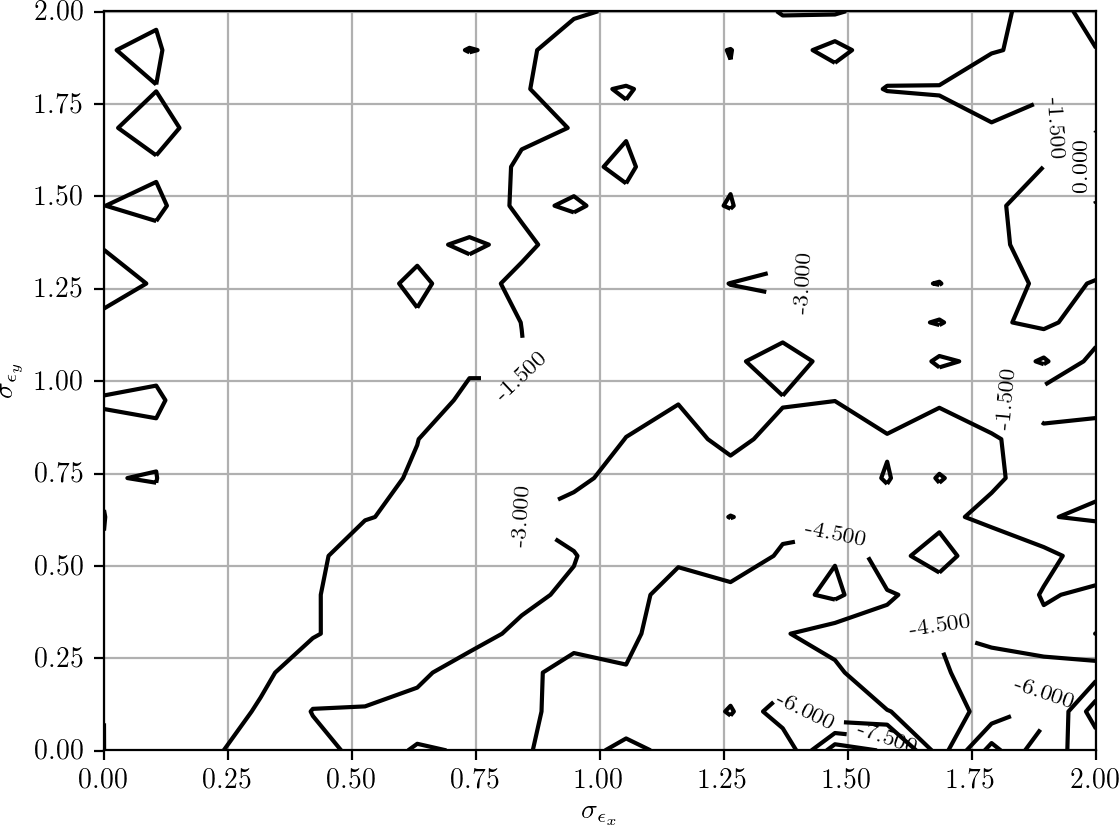
\includegraphics[width=135mm]{fig/nonlinear/quadratic/a-0_b-5_c-1.png}
    \caption{\( \theta_1 = 5 \)}\label{fig:comparison_nonlinear_quadratic_a-0_b-5_c-1}
  \end{subfigure}

  \vspace{\baselineskip}
  \caption{
    Точность оценивания параметров \\
    параболической модели при \( \theta_0 = 0, \theta_2 = 1 \)
  }\label{fig:comparison_nonlinear_quadratic_a-0_c-1}
\end{figure}

% \subsection{Обратная функция регрессии}

% Рассматривались функции регрессии вида
% \begin{equation*}
%   \psi = \theta_0 + \dfrac{1}{\theta_1 + \theta_2 \xi}.
% \end{equation*}

% На рисунках~\ref{fig:comparison_nonlinear_hyperbolic_a-0_b-0,001}--\ref{fig:comparison_nonlinear_hyperbolic_a-0_b-1}
% представлены графики функции \( d(\sigma_{\varepsilon_x}, \sigma_{\varepsilon_y}) \)
% для обратной функции регрессии \( \psi \) при
% различных значениях параметра \( \theta_2 \).
% {\color{red}Во всех описанных случаях оценивания параметров
% МРТ-оценки являются более точными.
% Кроме этого, отдельные оценки, полученные НМНК,
% являются совершенно неудовлетворительными,
% о чем свидетельствуют "пики" на приведенных графиках.
% }

% \begin{figure}[h]
%   \centering
%   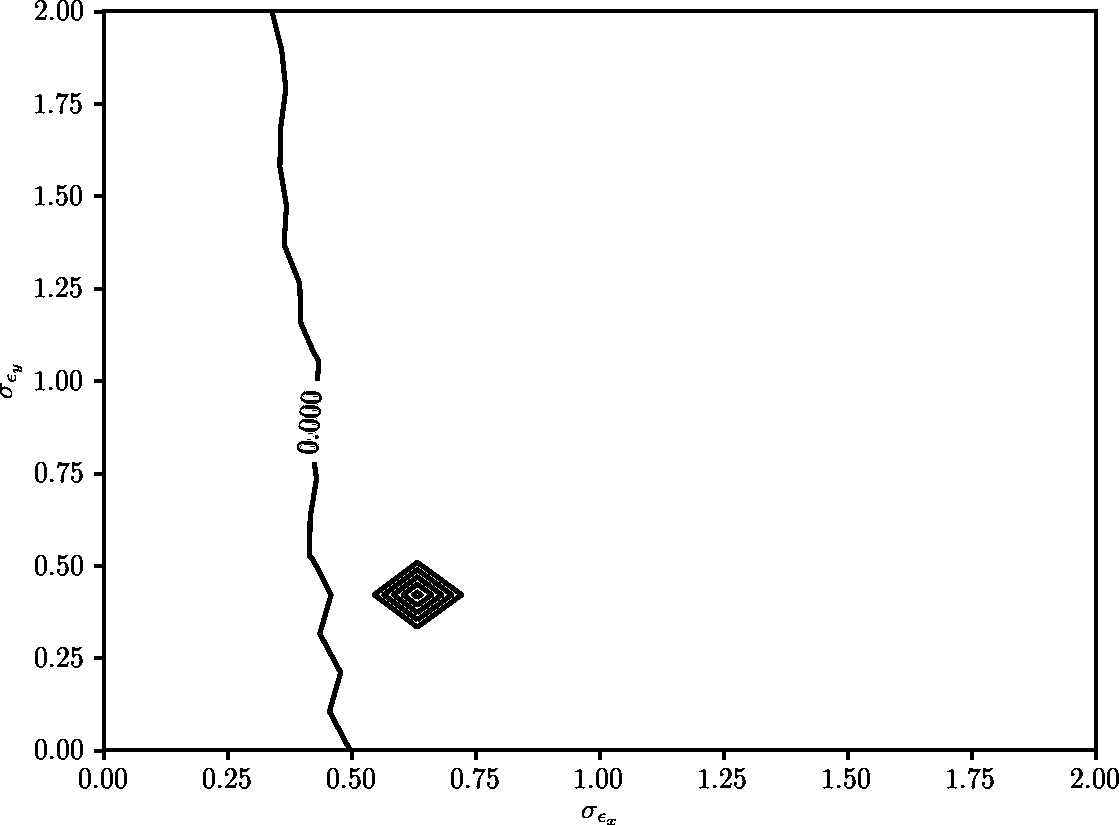
\includegraphics[width=135mm]{fig/nonlinear/hyperbolic/a-0_b-0,001.png}
%   \caption{
%     Точность оценивания параметров \\
%     гиперболической модели при \( \theta_1 = 0,001 \)
%   }\label{fig:comparison_nonlinear_hyperbolic_a-0_b-0,001}
% \end{figure}

% \begin{figure}[h]
%   \centering
%   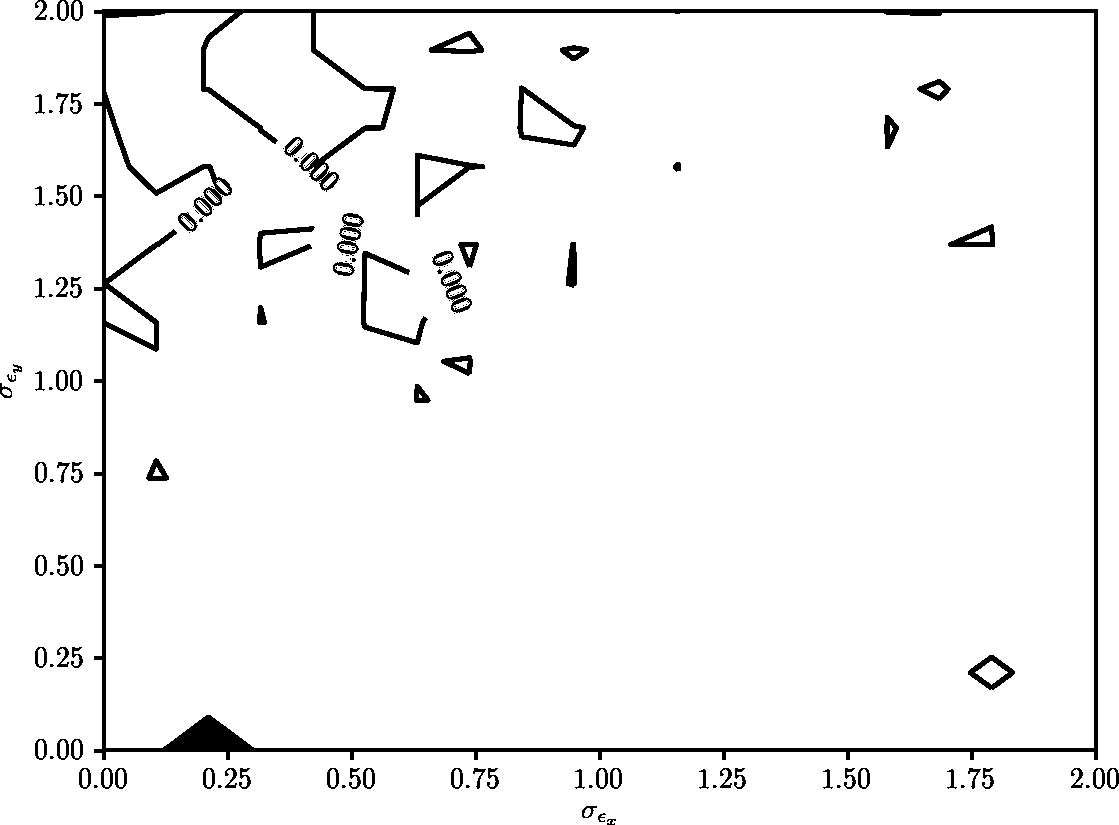
\includegraphics[width=135mm]{fig/nonlinear/hyperbolic/a-0_b-1.png}
%   \caption{
%     Точность оценивания параметров \\
%     гиперболической модели при \( \theta_1 = 1 \)
%   }\label{fig:comparison_nonlinear_hyperbolic_a-0_b-1}
% \end{figure}


% % \subsection{Экспоненциальная функция регрессии}
% % гиперболическая функция регрессии
% % степенная и показательная функции

% % \subsection{Степенная функция регрессии}

% % Рассматривались функции регрессии вида
% % \begin{equation*}
% %   \psi = \theta_1 \xi^{\theta_2}.
% % \end{equation*}


% % нелинейным регрессиям по оцениваемым параметрам
% \subsection{Синусоидальная функция регрессии}

% Рассматривались функции регрессии вида
% \begin{equation*}
%   \begin{aligned}
%     \psi_1 &= \theta_0 + \theta_1 \sin{0{,}2 \xi}, \\
%     \psi_2 &= \theta_0 + \theta_1 \sin{\xi}, \\
%     \psi_3 &= \theta_0 + \theta_1 \sin{5 \xi}.
%   \end{aligned}
% \end{equation*}

% На рисунках~\ref{fig:comparison_nonlinear_sinusoidal}
% представлены графики функции \( d(\sigma_{\varepsilon_x}, \sigma_{\varepsilon_y}) \)
% для синусоидальной функции регрессии \( \psi_2 \) при
% различных значениях параметра \( \theta_1 \).
% Во всех описанных случаях оценивания параметров
% НМНК-оценки являются более точными.
% Следует отметить, что при малых ошибках измерений выходной переменной
% нелинейный метод наименьших квадратов дает значительно более точные оценки.

% \begin{figure}[b]
%   \begin{subfigure}[b]{\linewidth}
%     \centering
%     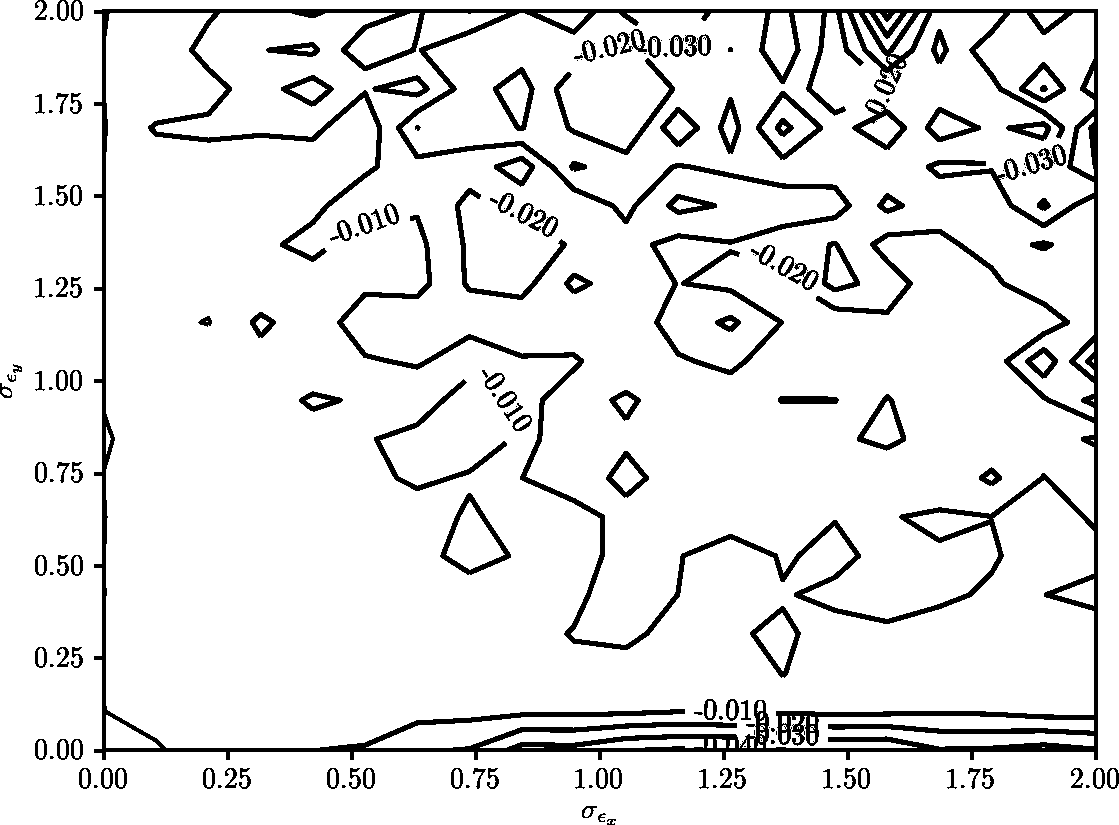
\includegraphics[width=135mm]{fig/nonlinear/sinusoidal/a-0_b-0,2.png}
%     \caption{\( \theta_1 = 0,2 \)}
%   \end{subfigure}

%   \vspace{2\baselineskip}
%   \begin{subfigure}[b]{\linewidth}
%   \centering
%   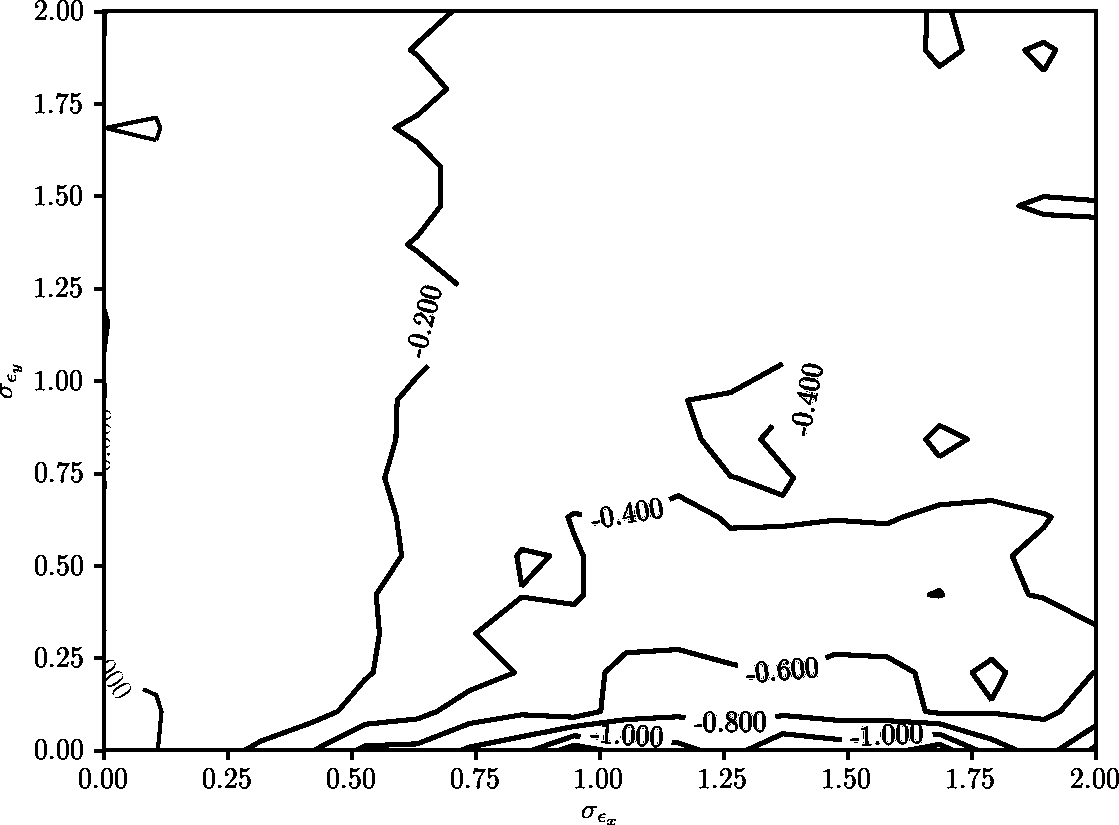
\includegraphics[width=135mm]{fig/nonlinear/sinusoidal/a-0_b-5.png}
%   \caption{\( \theta_1 = 5 \)}
% \end{subfigure}

% \vspace{\baselineskip}
%   \caption{
%     Точность оценивания параметров \\
%     синусоидальной модели
%   }\label{fig:comparison_nonlinear_sinusoidal}
% \end{figure}

%
% Точность НМНК существенным образом зависит от того, насколько удачной оказалась опорная оценка.
% В некоторых случаях получить хорошую опорную оценку проблематично.
% МРТ не зависит от опорных оценок и дает хорошие результаты там, где НМНК дает осечку.
% Предлагается использовать МРТ-оценку в качестве опорной для НМНК.
%